\section{Abstract}
In diesem Versuch werden die Eigenschaften von Mikrowellen und den Bauteilen der Hochfrequenztechnik untersucht. Zuerst wird die Kennlinie der verwendeten Messdiode bestimmt, um damit die Leistung der Mikrowellen im weiteren Versuch bestimmen zu können. Anschließend werden bei einem Zirkulator, einem Isolator und einem Richtkoppler Dämpfungen in Abhängigkeit der Frequenz gemessen. Zuletzt werden in zwei verschiedenen Koaxialkabeln stehende Wellen erzeugt, welche über die dabei entstehenden Resonanzen nachgewiesen werden. Anschließend werden aus den Frequenzabständen zwischen den Resonanzen die Lichtgeschwindigkeit im Koaxialkabel und die relative Permittivität der Kabel bestimmt.

\section{Theorie}
\subsection{Hilfseinheit Bel}
In der Leitungstheorie werden oft relative Größen betrachtet, daher wurde die Hilfseinheit Bel eingeführt. Hiermit lässt sich das Verhältnis zwischen zwei Energiegrößen, das Relativmaß $R$ (siehe \cref{eq:R}), im dekadischen Logarithmus ausdrücken. Meistens wird hier die Einheit Dezibel verwendet, die einem zehntel Bel entspricht.

\begin{equation}
	R = \log_{10} \left( \frac{P_2}{P_1}\right) \text{B} =10 \log_{10} \left( \frac{P_2}{P_1}\right) \text{dB}
	\label{eq:R}
\end{equation}

Auch absolute Größen können in Dezibel angegeben werden. Dazu wird für $P_1$ ein Referenzwert eingesetzt. Dies ist sinnvoll bei Größen, deren Werte in verschiedenen Größenordnungen liegen. Ein Größe, die häufig auf diese Weise angegeben wird, ist der Leistungspegel (siehe \cref{eq:Lp}). Dabei ist der Referenzwert $\SI{1}{mW}$ und die Einheit dBm.

\begin{equation}
	L_P = 10\log_{10}\left( \frac{P}{1\text{mW}}\right) \text{dBm}
\end{equation}

\subsection{Grundlagen der Leitungstheorie}
\subsubsection{Stationäre Leitungsgleichungen}
Mikrowellen können mithilfe der Maxwell-Gleichungen als elektromagnetische Wellen mit E- und B-Feld betrachtet werden. Bei sogenannte TEM-Leitern (transversalelektromagnetische Leiter) erfüllen diese Felder bestimmte Randbedingungen an Grenzflächen und können daher auf die Größen $I$ und $U$ reduziert werden. TEM-Leiter bestehen immer aus einem Hin- und Rückleiter. Außerdem werden stationäre Zustände betrachtet, sodass Einschwingvorgänge keine Rolle spielen. In \cref{ersatz} ist das Ersatzschaltbild eines homogenen Leiterabschnitts der Länge $\Delta x$ dargestellt. Dieser Abschnitt lässt sich durch vier Impedanzen beschreiben.

\begin{figure}[h]
	\centering
	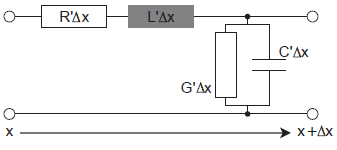
\includegraphics[width=0.9\textwidth]{Ersatzschaltbild.png}
	\caption{Ersatzschaltbild eines homogenen Leitungsabschnitts mit Länge $\Delta x$.}
	\label{ersatz}
\end{figure}

Diese werden als Beläge definiert. Bei verlustlosen Leitungen sind dies der Induktivitätsbelag $L'$ und der Kapazitätsbelag $C'$. Bei verlustbehafteten Leitungen spielen ebenfalls der Widerstandsbelag $R'$ und der Ableitungsbelag $G'$ eine Rolle. Die Übertragungsfunktion dieses LTI-Systems (lineares zeitinvariantes System) lässt sich über die Kirchhoffschen Regeln (\cref{eq:masche} und \Cref{eq:knoten}) bestimmen, wobei $G' \Delta x$ das Inverse eines Widerstands ist.

\begin{equation}
	\text{Maschenregel}: U(x + \Delta x) - U(x) = -(R' + i\omega L')I(x) \Delta x
	\label{eq:masche}
\end{equation}

\begin{equation}
	\text{Knotenregel}: I(x + \Delta x) - I(x) = -(G' + i\omega C')U(x) \Delta x
	\label{eq:knoten}
\end{equation}

Daraus lassen sich nun die stationären Leitungsgleichungen (\cref{eq:sl1} und \cref{eq:sl2}) aufstellen.

\begin{equation}
	\frac{\text{d}U(x)}{\text{d}x} = -(R' + i\omega L')I(x)
	\label{eq:sl1}
\end{equation}

\begin{equation}
	\frac{\text{d}I(x)}{\text{d}x} = -(G' + i\omega C')U(x)
	\label{eq:sl2}
\end{equation}

Diese können mit einem Ansatz, bei dem eine hinlaufende ($U_h$)und eine rücklaufende ($U_r$) Welle betrachet werden, gelöst werden. (siehe \cref{eq:i} und \cref{eq:u})

\begin{equation}
	I(x) = I_h e^{-\gamma x} + I_r e^{\gamma x}
	\label{eq:i}
\end{equation}

\begin{equation}
U(x) = U_h e^{-\gamma x} + U_r e^{\gamma x}
\label{eq:u}
\end{equation}

\begin{equation*}
	\text{mit} \gamma = \sqrt{(R' + i\omega L')(G' + i\omega C')}
\end{equation*}

\subsubsection{Wellenwiderstand}
An \cref{eq:sl1} und \cref{eq:sl2} wird deutlich, dass Spannung und Stromstärke über einen frequenzabhängigen Faktor voneinander abhängen, den sogenannten Wellenwiderstand $Z_\text{L}$. Anhand von \cref{eq:zl} ist erkennbar, dass der Wellenwiderstand nur von den Belägen, also der Geometrie und dem Material des Leiters, abhängt.

\begin{equation}
	Z_\text{L} = \frac{U(x)}{I(x)} = \sqrt{\frac{R' + i\omega L'}{G' + i\omega C'}}
	\label{eq:zl}
\end{equation}

Betrachtet man den einfachen Fall einer verlustfreien Leitung, ergibt sich:

\begin{equation}
	Z_\text{L} = \sqrt{\frac{R'}{C'}}
	\label{eq:zl2}
\end{equation}

\subsubsection{Reflexionskoeffizient}
Bei TEM-Leitern treten immer ein hinlaufende und eine rücklaufende Welle auf. Die hinlaufende Welle ist das zu übertragene Signal, die rücklaufende Welle ist meist eine unerwünschte Reflexion. Die Reflexion findet dabei am Kabelende statt und wird durch \cref{eq:reflexion} beschrieben.

\begin{equation}
	r = \frac{Z_a - Z_L}{Z_a + Z_L}
	\label{eq:reflexion}
\end{equation}

$Z_a$ ist hier der Abschlusswiderstand. Das Kabel wird als abgeschlossen bezeichnet, wenn  $Z_a = Z_L$. Für den Grenzfall eines offenen Kabelendes geht $Z_a$ gegen $\inf$ und daher $r$ gegen $1$. Beim Grenzfall eines kurzgeschlossenen Kabels geht dagegen $Z_a$ gegen $0$ und $r$ gegen $-1$.

\subsubsection{Stehende Wellen}
Existieren eine hinlaufende und eine rücklaufende Welle gleicher Frequenz, bilden sie eine stehende Welle. Diese hat Knotenpunkte, deren Position zeitlich konstant ist. Für diese Art von Welle muss im Leiter Reflexion stattfinden. Die Amplitude der stehenden Welle ist abhängig vom Reflexionskoeffizienten. Tritt vollständige Reflexion auf, also $r=1$, dann bildet sich eine ideale stehende Welle, ansonsten bilden sich Wanderwellen.

\subsubsection{Mehrfachreflexion}
Mehrfachreflexionen treten auf, wenn die Abschlusswiderstände an Kabeln falsch gewählt sind oder am Kabel selbst Defekte auftreten. Durch die Reflexion tritt Interferenz zwischen den verschieden häufig reflektierten Wellen gleicher Frequenz auf. Interferieren die Wellen konstruktiv miteinander entsteht eine Resonanz. Die transmittierte Leistung einer verlustlosen Leitung lässt sich dann mit \cref{eq:trans} beschreiben.

\begin{equation}
	P_t = \frac{|U_h|^2}{Z_L}\left( \frac{T}{1-R}\right) ^2 \frac{1}{1 + F \sin^2\left( \frac{\Phi}{2}\right) }
	\label{eq:trans}
\end{equation}

Dabei ist $T$ der Transmissionkoeffizient, $R$ der Reflexionskoeffizient und $F$ der Finesse Faktor (siehe \cref{eq:finesse}).

\begin{equation}
	F = \frac{4R}{\left( 1-R\right) ^2}
	\label{eq:finesse}
\end{equation}

\cref{eq:trans} bezeichnet man als Airy-Funktion. Damit kann das Transmissionsverhalten eines optischen Resonators beschrieben werden. Wenn Reflexionskoeffizient und Transmissionkoeffizient konstant sind, dann wird die transmittierte Leistung offenbar maximal, wenn der Sinus in \cref{eq:trans} verschwindet. Daraus folgt für $\Phi$:

\begin{equation}
	\Phi = 2\pi n
\end{equation}

Die meiste Leistung wird also reflektiert, wenn

\begin{equation}
	2 k_n l - \phi_1 -\phi_2 = 2\pi n
\end{equation}

erfüllt ist, wobei $\phi_1$ und $\phi_2$ die Phasensprünge sind, um die die Welle and er jeweiligen Stelle reflektiert wird. Während des Durchgangs durch den Resonator muss die Welle also für Resonanz eine Phase zurücklegen, die ein ganzzahliges Vielfaches von $2\pi$ ist.

\subsection{Bauteile der Hochfrequenztechnik}
\subsubsection{Koaxialkabel}
Der Aufbau eines Koaxialkabels ist in \cref{Koax} abgebildet. Der Koaxialkabel besteht aus einer Innen- sowie einer Außenleitung. Zwischen beiden Leitungen liegt ein ein Dielektrikum. Dieses führt dazu, dass sich das elektromagnetische Feld im Leiter befindet. Der Widerstand, welcher durch Abstrahlung einer elektromagnetischen Welle erzeugt wird, wird dadurch verringert. 
\begin{figure}[h]
	\centering
	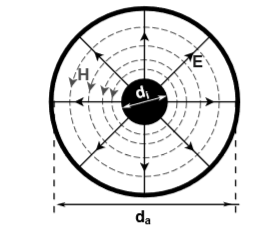
\includegraphics[scale=1]{Koaxial.png}
	\caption{Aufbau eines Koaxialkabel. Dabei ist das E-Feld (E) und das magnetische Feld (H) innerhalb der Innen- und Außenleitung. Der Durchmesser beider Leitungen ist durch $d_a$ und $d_i$ dargestellt.}
	\label{Koax}
\end{figure}
Wenn die relative Permittivität ($\epsilon_r$) und der Außen- ($d_i$) sowie Innenradius ($d_a$) bekannt ist, kann in dem nahezu homogenen elektrischen Feld eine Kapazität (C) und eine Induktivität definiert werden.
\begin{align*}
	C &= 2 \pi \epsilon_0 \epsilon_r \frac{1}{\ln{\frac{d_a}{d_i}}} \\
	L &= \frac{\mu_0 \mu_r }{2 \pi} \ln{\frac{d_a}{d_i}}
\end{align*}
Dabei stellt $\mu_0$ und $\mu_r$ die magnetische Feldkonstante im Vakuum bzw. im Material.

\subsubsection{Mikrostreifenleitung}
In \cref{Mikrostreifen} ist der Aufbau einer Mikrostreifenleitung zu sehen. Dieser besteht aus einem schmalen metallischen Streifen, welcher auf einem Dielektrikum verbaut ist. Unterhalb des Dieelektrikums befindet sich eine Platine.
\begin{figure}[h!]
	\centering
	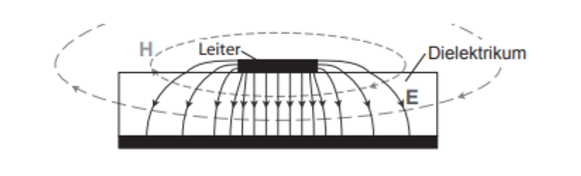
\includegraphics[scale = 1]{mikrostreifen.png}
	\caption{Aufbau eines Zirkulators}
	\label{ZB}
\end{figure}
Der Vorteil dieser Technik ist, dass der Aufbau klein gegenüber eines Koakialkabels ist. Der Nachteil ist, dass das elektomagnetische Feld teilweise außerhalb der Vorrichtung liegt. Somit entsteht ein größerer Verlust. Ebenfalls ist die Vorrichtung störanfälliger.

\subsubsection{Zirkulator}
Ein Zirkulator ist ein Dreitor, welches eine stehende Welle nach dem Prinzip in \cref{ZB} weiterleitet.
\begin{figure}[h!]
	\centering
	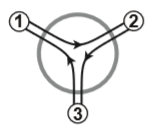
\includegraphics[scale = 1]{Zirk-Bild.PNG}
	\caption{Aufbau eines Zirkulators}
	\label{ZB}
\end{figure}
Bei einem idealen Zirkulator geht der gesamte Stromfluss ohne Verlust  durch den Zirkulator hindurch. Somit tritt kein Energieverlust zwischen den Toren auf. Die gesamte Energie von Tor 1 tritt an Tor 2 aus. Analog der Pfeile tritt die gesamte Energie, die in Tor 2 bzw. in Tor 3 einläuft, bei Tor 3 bzw. bei Tor 1 aus. Wichtige Größen zur Charkterisierung des Zirkulators sind die Bandbreite, die Durchlassdämpfung und die Sperrdämpfung.

\begin{align}
	\text{Durchlassdämpfung} = 10 \cdot \ln{\frac{P_1}{P_2}}dB \\
	\text{Sperrdämpfung} =  10 \cdot \ln{\frac{P_1}{P_3}}dB 
\end{align}

\subsubsection{Isolator}
Ein Isolator ist ein Zirkulator, welcher an Tor 3 ein angepassten Abschlusswiderstand besitzt. Das führt dazu, dass ein Isolator eine Welle in eine Richtung nahezu durchlässt, wohingegen es die Welle in entgegengesetzter Richtung absorbiert. Sie werden genutzt um Mikrowellengeneratoren vor Reflexion zu schützen.

\subsubsection{Richtkoppler}
Ein Richtkoppler ermöglicht es Wellen mit verschiedenen Ausbreitungsrichtungen voneinander zu trennen. Das kann dazu dienen, dass man die einzelnen Wellen messen kann. Ein Richtkoppler ist ein Viertor. Somit besitzt er vier Ein- bzw. Ausgänge. Der schematische Aufbau eines Richtkopplers findet man in \cref{RB}. 
\begin{figure}[h!]
	\centering
	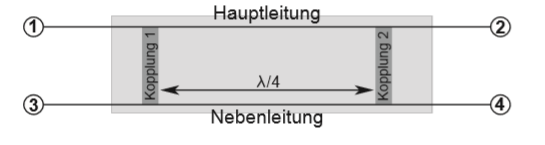
\includegraphics[scale = 1]{Richt-Bild.PNG}
	\caption{}
	\label{RB}
\end{figure}
Der Richtkoppler ist in eine Hauptleitung und in eine Nebenleitung eingeteilt. Er funktioniert über das Prinzip von konstruktiver und destruktiver Interferenz. Dazu werden die Haupt- und Nebenleitungen über einen Wellenleiter mit  einer Länge von $\frac{\lambda}{4}$ verbunden. Betrachten wir den Fall,dass eine Welle in Tor 1 ein läuft, so spaltet sich die Welle im ersten Kopplungspunkt in zwei Teilwellen auf. Einmal folgt die Welle der Hauptleitung und einmal wird diese auf die Nebenleitung übertragen. Bis die Welle die Nebenleitung erreicht, vergeht eine Länge von $\frac{\lambda}{4}$. Ebenso vergeht eine Länge von $\frac{\lambda}{4}$, bis die Welle den zweiten Kopplungspunkt auf der Hauptleitung erreicht. Hier spaltet sich die Welle wieder auf und benötigt wiederum eine Länge von $\frac{\lambda}{4}$ um die Nebenleitung zu erreichen. Wenn jetzt eine Welle von Tor 1 zu Tor 4 betrachtet wird, kann aufgrund von konstruktiver Interferenz ein Leistungsübertrag beobachtet werden, wohingegen bei einer Welle von Tor 1 zu Tor 3 eine destruktive Interferenz beobachtet wird. Das hängt damit zusammen, da die Welle im zweiten Fall genau eine Wellenlängenänderung von $\frac{\lambda}{2}$ erfährt.
Wie viel Leistung der Hauptleitung auf die Nebenleitung übertragen wird hängt von der Stärke der Kopplung ab. Sie wird durch die Koppeldämpfung beschrieben.
\begin{align}
	\text{Koppeldämpfung} = 10\cdot \ln{\frac{P_1}{P_4}}dB
	\label{KppF}
\end{align}
Die Isolation gibt an wie viel der Welle von Tor 1 ungewollt an Tor 3 ausgegeben wird.
\begin{align}
	\text{Isolation} = 10\cdot \ln{\frac{P_2}{P_4}}dB
	\label{IsoF}
\end{align}
Die Dämpfung auf der Hauptleitung gibt die Einfügedämpfung an. 
\begin{align}
	\text{Einfügedämpfung} = 10\cdot \ln{\frac{P_1}{P_2}}dB
	\label{EinF}
\end{align}


\subsubsection{Diode bzw. Detektor}
Für die verwendeten Messgeräte ist es notwendig die Mikrowellen vor dem Messen gleich zu richten. Dafür wird eine Diode verwendet. In einer Richtung ist die Diode in Durchlassrichtung geschaltet, wohingegen in die entgegen gesetzte Richtung die Diode in Sperrrichtung geschaltet ist. So lässt diese nur eine Stromrichtung zu.
Es gibt mehrere Arten von Dioden. Eine Art ist die Halbleiter-Halbleiter-Diode.
Die Halbleiter-Halbleiter-Dioden beruhen auf dem Prinzip, dass eine p- und eine n-Dotierte Schicht vorliegt. Die p-Dotierte Schicht senkt das Ferminiveau des Leiters, wohingegen die n-Dotierte Schicht das Ferminiveau anhebt. Wenn beide Materialien zusammengebracht werden, gleicht sich das Ferminiveau aus und es entsteht in der Mitte des Halbleiters eine Raumladungszone, in der ein elektrisches Feld existiert. Wenn nun eine äußere Spannung mit Pluspol am p-dotierten Halbleiter angelegt wird, vergrößert sich die Raumladungszone und es kann kein Strom fließen. Falls der Pluspol am n-dotierten Übergang angelegt wird, wird das innere Elektrische Feld abgebaut und es entsteht ein Stromfluss.
Eine andere Methode eine Diode zu bauen, ist die Möglichkeit der Schottky-Diode. Diese Dioden reagieren schneller. Schottky-Dioden sind Metall-Halbleiter-Dioden. Anstelle des p-dotierten Halbleiters tritt eine Metallelektrode auf. Somit liegt das Ferminiveau oberhalb der Standartnorm. Diese wirkt alleine für die Sperrschicht. 


\section{Methoden und Durchführung}
Zur Erzeugung der Mikrowellen wird ein Mikrowellengenerator Wiltron 6759B verwendet. Die Wellen werden dann durch Koaxialkabel und verschiedene Bauteile geleitet. Anschließend werden sie an einer Messdiode (Schottky-Diode) in Gleichstrom umgewandelt, dessen Spannung von einem Digitalmultimeter TTi 1906 gemessen wird. Die Spannung ist dabei abhängig von der Leistung der Mikrowellen.
\subsection{Kennlinie}
Zuerst soll die Kennlinie der Diode bestimmt werden. Dazu wird diese nach \cref{Aufbau} gemessen. Dabei wird die die Leistung der Mikrowellenstrahlung in Spannung umgewandelt. Dies wird auch in allen weiteren Messungen verwendet, da sich die Spannung einfacher direkt messen lässt.

\begin{figure}[h]
	\centering
	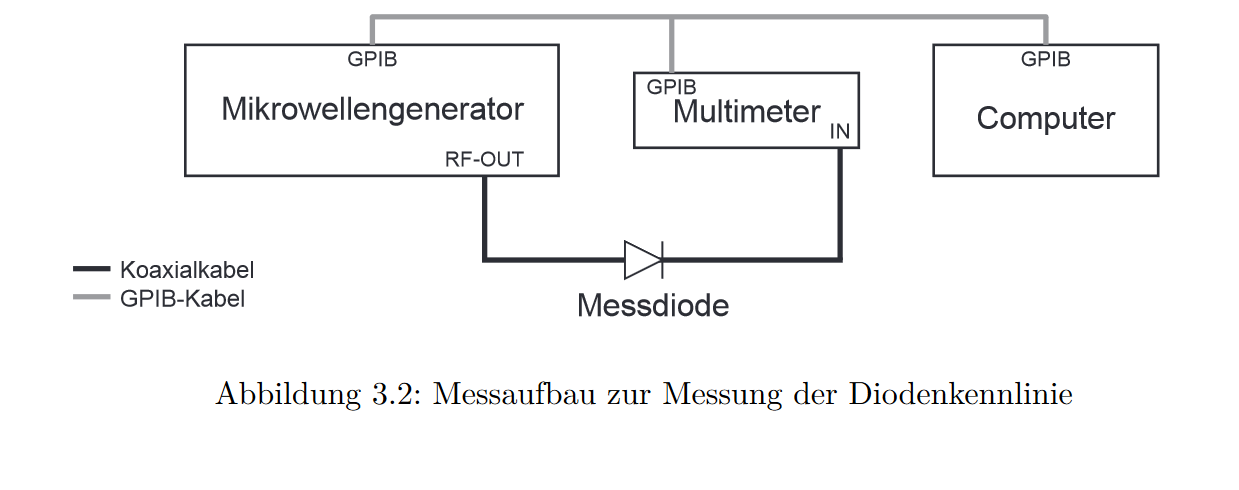
\includegraphics[scale=0.4]{Diode_Aufbau.PNG}
	\caption{Skizze des Versuchaufbaus}
	\label{Aufbau}
\end{figure}

\subsection{Messung der Bauteile}
Um die Bauteile zu messen wird die Apparatur in \cref{Mess} verwendet.
\begin{figure}[h!]
	\centering
	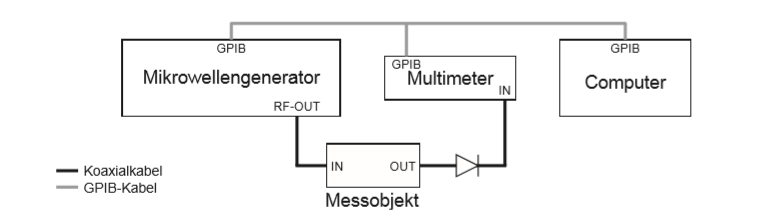
\includegraphics[scale = 1]{Mess.png}
	\caption{}
	\label{Mess}
\end{figure}
Der Aufbau ähnelt dem vom vorherigen Versuch zur Bestimmung der Diodenkennnlinie. Jetzt wird ein Messobjekt zwischen dem Mikrowellengenerator und der Diode eingebaut. Zuerst betrachten wir ein Isolator, danach ein Zirkulator und zum Schluss einen Richtkoppler. Zum messen all dieser Bauteile wird ein vorprogrammiertes LabVIEW Programm benutzt. Dieses zeichnet die Spannung in Abhängigkeit von der Frequenz auf. Die Messwerte werden in Dämpfung pro Frequenz aufgetragen, sodass die folgende Umrechnung erfolgen muss, wobei P die Leistung darstellen soll.
\begin{align}
	\text{dB} = 10\text{dBm} - \text{P}
	\label{F1}
\end{align}

\subsection{Ausbreitungsgeschwindigkeit und relative Permittivität}
Zuletzt sollen in zwei verschiedenen Koaxialkabeln stehende Wellen erzeugt und die Resonanzfrequenzen, bei denen die stehenden Wellen beobachtet werden, gemessen werden. Aus den Abständen zwischen den Resonanzen soll anschließend mit \cref{eq:c} die Ausbreitungsgeschwindigkeit der Welle im Kabel berechnet werden.
\begin{equation}
c = 2l(f_{n+1} - f_n)
\label{eq:c}
\end{equation}
Zuletzt soll dann mit \cref{eq:er} die relative Permittivität bestimmt werden.
\begin{equation}
\epsilon_r = \left( \frac{c_0}{c}\right) ^2
\label{eq:er}
\end{equation}

\section{Auswertung}
\subsection{Kennlinie}
Zuerst wird die Kennlinie der Diode bestimmt. Diese wird in \cref{fuck_scidavis} dargestellt. Dabei wird mit einer e-Funktion gefittet, durch die beschrieben wird, welche Leistung in wie viel Spannung umgewandelt wird. 

\begin{figure}[h]
	\centering
	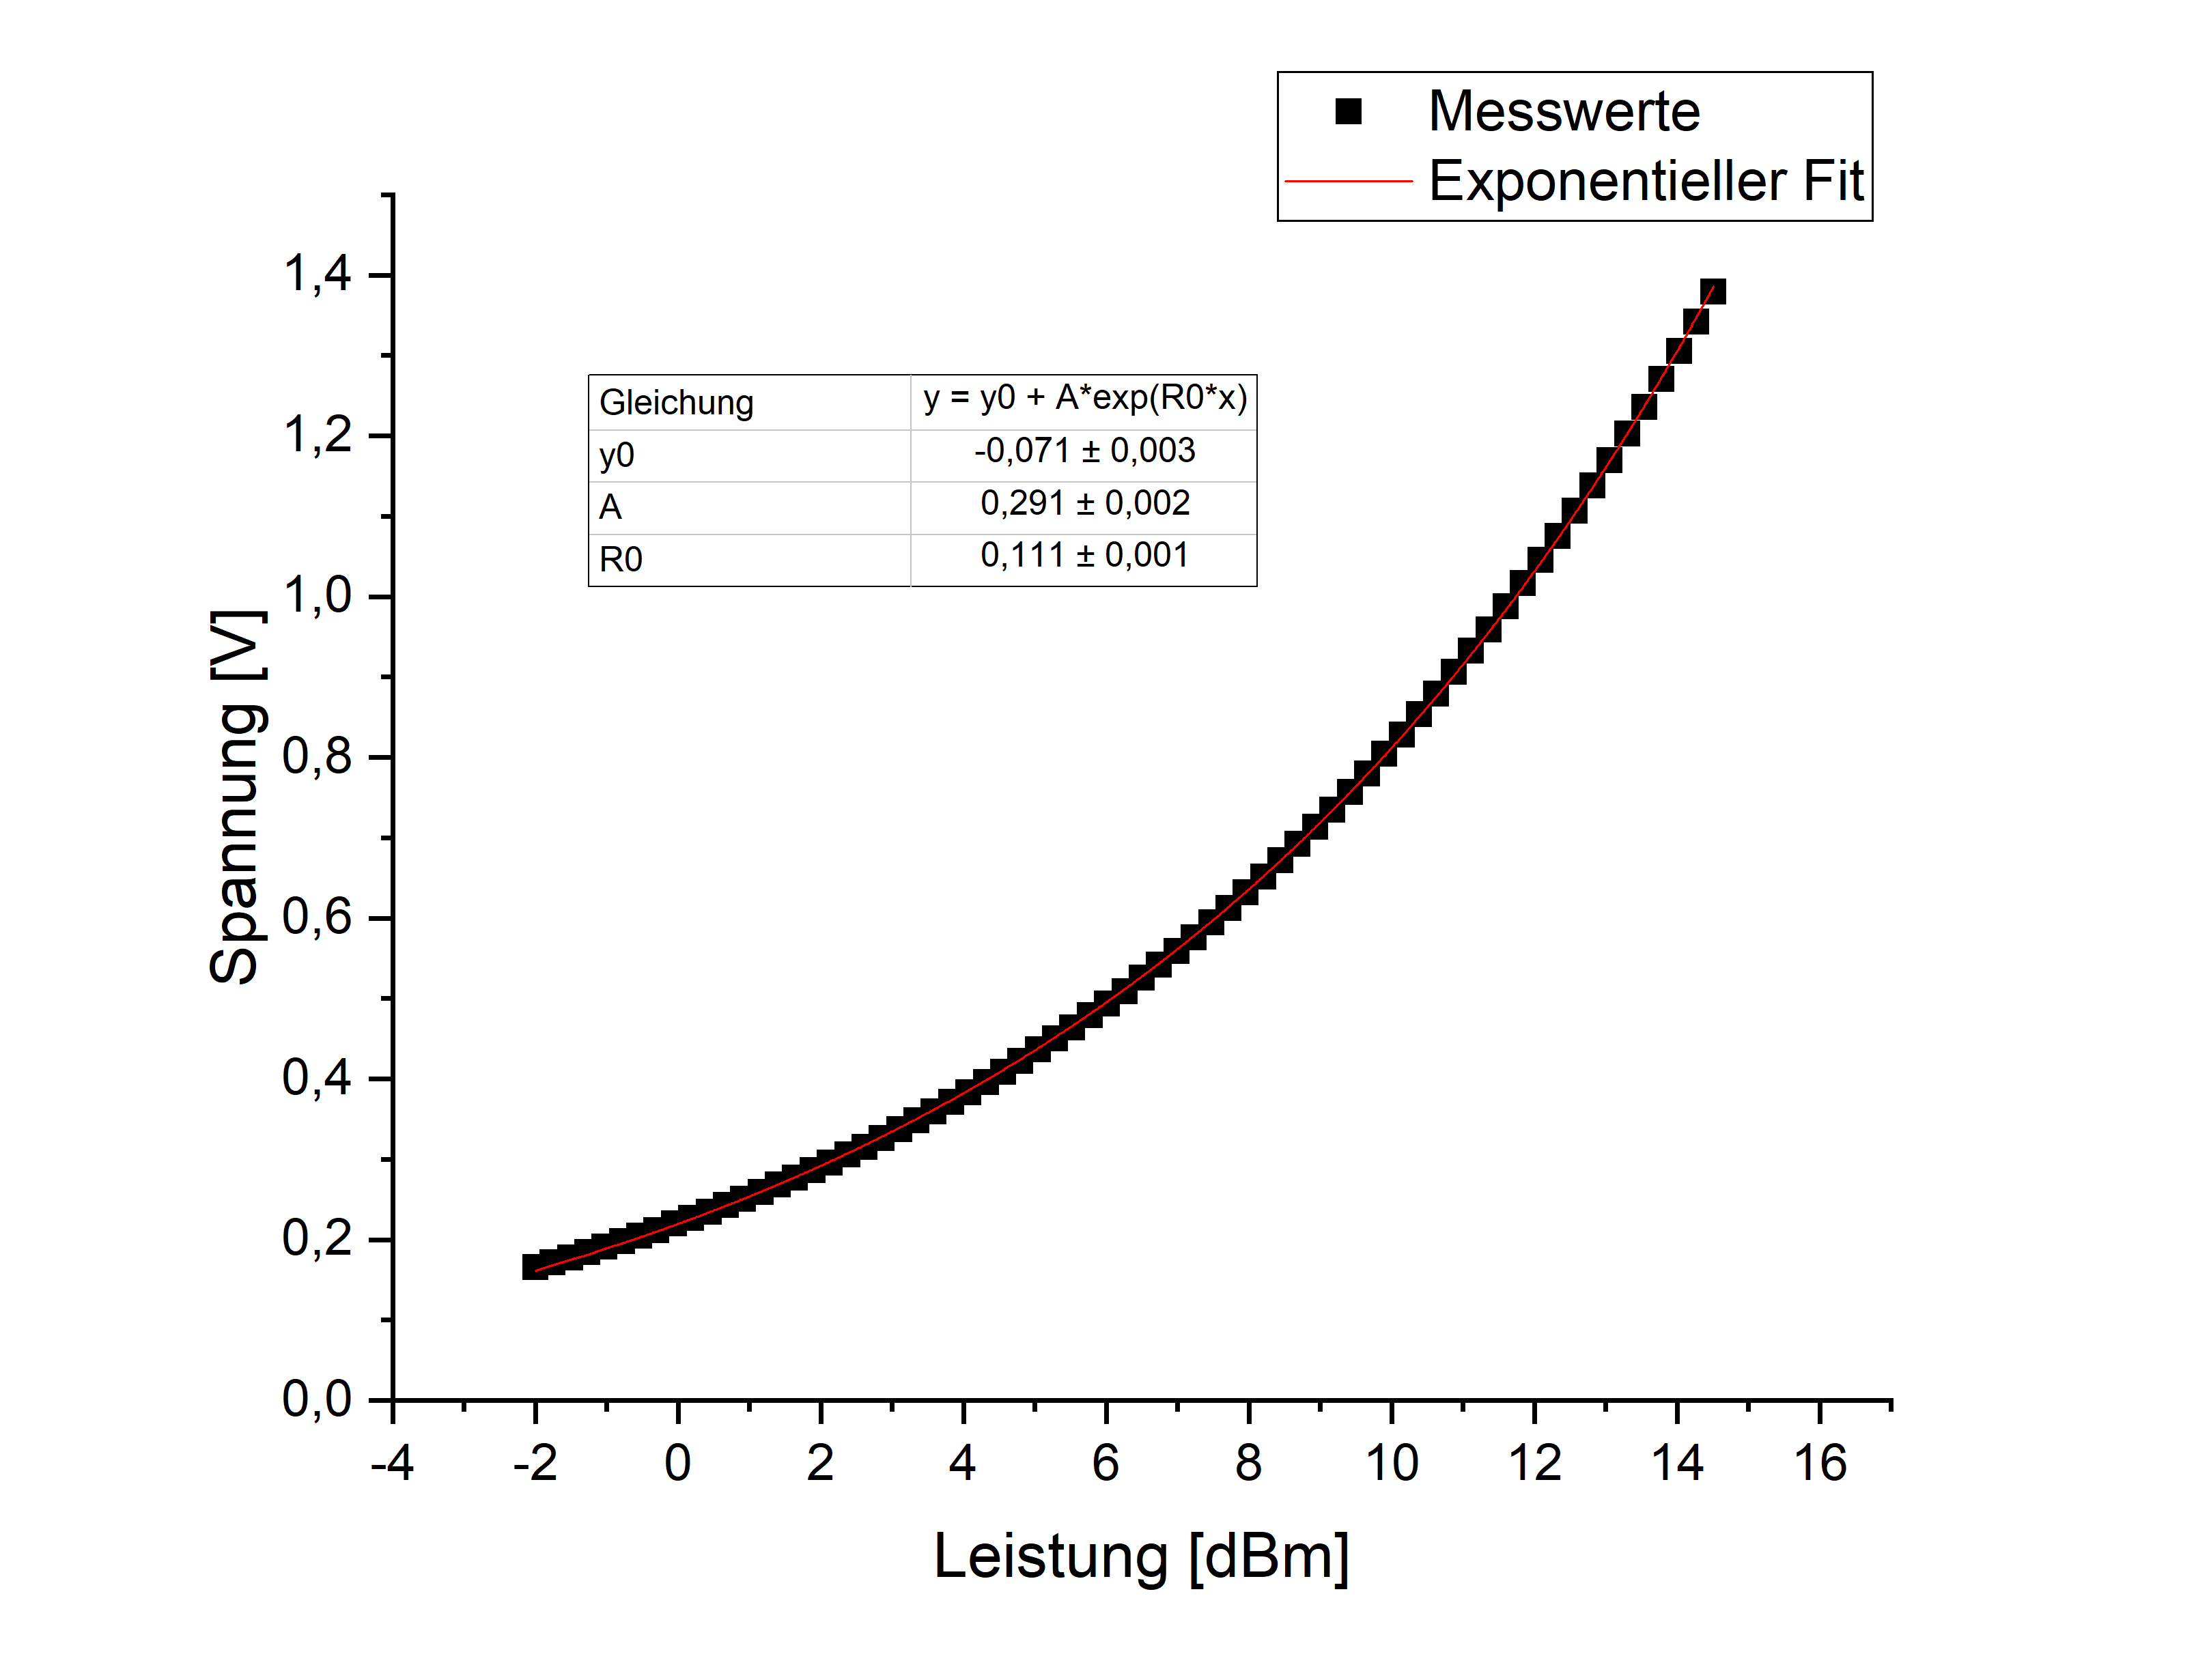
\includegraphics[scale=0.4]{fuck_scidavis.PNG}
	\caption{Kennlinie der Diode}
	\label{fuck_scidavis}
\end{figure}

\subsection{Bauteile der Hochfrequenztechnik}
In diesem Teil werden die Dämpfungen der Bauteile in Abhängigkeit der Frequenz dargestellt. Da in allen Messungen die Spannung in Abhängigkeit der Frequenz dargestellt wird, muss die Spannung zunächst mit der Formel der Diodenkennlinie in Leistung umgerechnet werden. Die Umrechnung von Leitung in Dämpfung erfolgt über \cref{F1}. Alle Grafiken wurden mit dem Programm OriginPro erstellt.
\subsubsection{Isolator}
In \cref{Isolator} ist die Dämpfung in Abhängigkeit der Frequenz dargestellt. Wie erwartet besitzt die Sperrrichtung einen höheren Dämpfwert als die Durchlassrichtung. Innerhalb eines bestimmten Bereiches kann die Dämpfung als konstant angesehen werden außerhalb des Bereiches weißt die Kurve ein nicht lineares Verhalten auf. Es wird nur der Bereich charakterisiert, welcher ein nahezu lineares bzw. konstantes Verhalten aufweist.
\begin{figure}[h!]
	\centering
	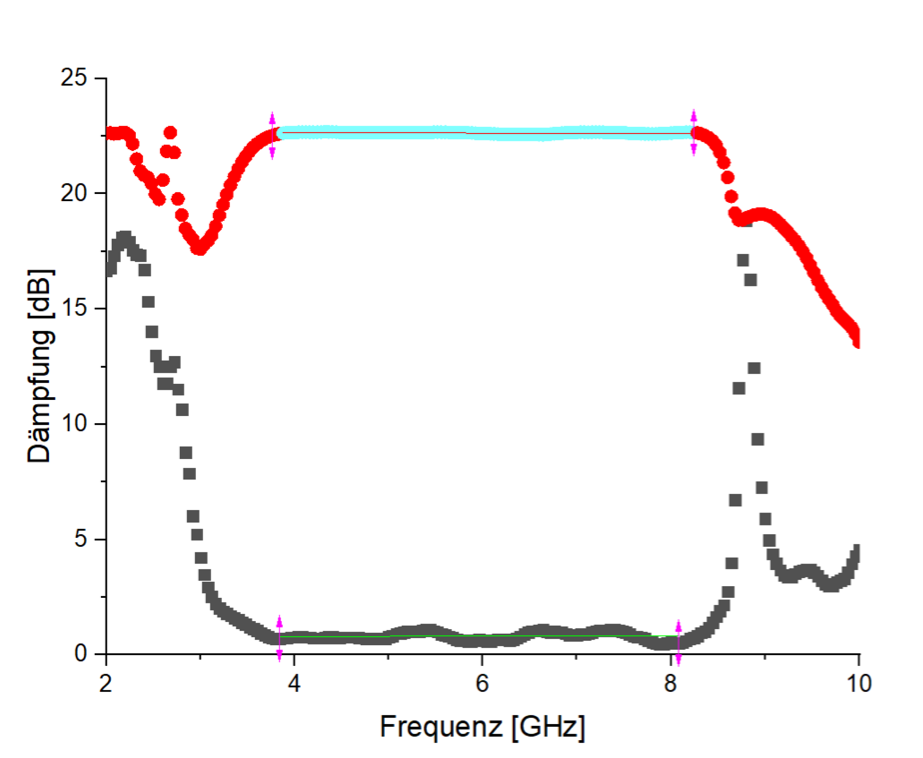
\includegraphics[scale = 1]{Isolator11.png}
	\caption{Die roten Punkte stellen die Sperrdämpfung dar. Das Intervall mit den türkisen Punkten stellt die Bandbreite sowie den ausgewerteten Bereich dar. Die schwarzen Punkte stellen die Durchlassdämpfung dar. Über die rosa Markierungen wurde der gefittete Bereich dargestellt. Dieser Bereich entspricht der Bandbreite. Die vorliegenden Fits entsprechen linearen Fits von der Form $y = a + bx$. Die Fitparameter in Sperrichtung sind $a = (22,70 \pm 0,02)$dB und $b = (-0,009 \pm 0,002)$dB/Ghz. Die Fitparameter in Durchlassrichtung betragen $a = (0,77 \pm 0,08)$dB und $b = (-0,01 \pm 0,01)$dB/GHz.}
	\label{Isolator}
\end{figure}
Die Bandbreite beider Dämpfungen befinden sich bei etwa 4Ghz bis 8Ghz. Anhand der vom Fit bestimmten Parameter, ist bei der Durchlassrichtung der erwartete konstante Verlauf bestätigt worden. Wenn die Grafik genauer betrachtet wird, können Wellen innerhalb der Messwerte beobachtet werden. Diese Wellen können dadurch entstanden sein, dass der Koaxialkabel der zwischen dem Mikrowellengenerator und dem Messobjekt befestigt worden ist relativ kurz war und eine starke Biegung an einer Stelle aufgewiesen hat. Genau an dieser Stelle konnte es bei einigen Frequenzen zur Reflexion kommen, sodass der Koaxialkabel ein Reflexionsanteil besessen hat, der sich negativ zum Durchlassvermögen auswirkte. Diese Ungenauigkeit wurde bei den flgenden Versuchen korrigiert, indem man ein längeres Kabel verbaut hat, welches keine starke Krümmung aufgewiesen hat. Bei der Sperrichtung ist ebenfalls ein nahezu konstanter Verlauf zu beobachten. Hier kann jedoch nicht innerhalb der Messunsicherheiten zu einem Konstanten Verlauf geschlossen werden. Die Steigung ist jedoch so gering, dass dies durch nicht berücksichtigte Unsicherheiten des Aufbaus zustande gekommen sein könnte. Mit Hilfe der Plots kann eine Dämpfung angegeben werden. Für die Durchlassrichtung beträgt die Dämpfung $a = (0,77 \pm 0,08)$ dB und die Dämpfung in Sperrichtung beträgt
$a = (22,70 \pm 0,02)$dB.

\subsubsection{Richtkoppler}
Als nächstes wird der Richtkoppler betrachtet. In \cref{Richt} ist die Isolation, die Koppeldämpfung und die Einfügedämpfung dargestellt. Dabei besitzt die Isolation die stärkste Dämpfung. Danach kommt die Koppeldämpfung und danach die Einfügedämpfung.
\begin{figure}[h!]
	\centering
	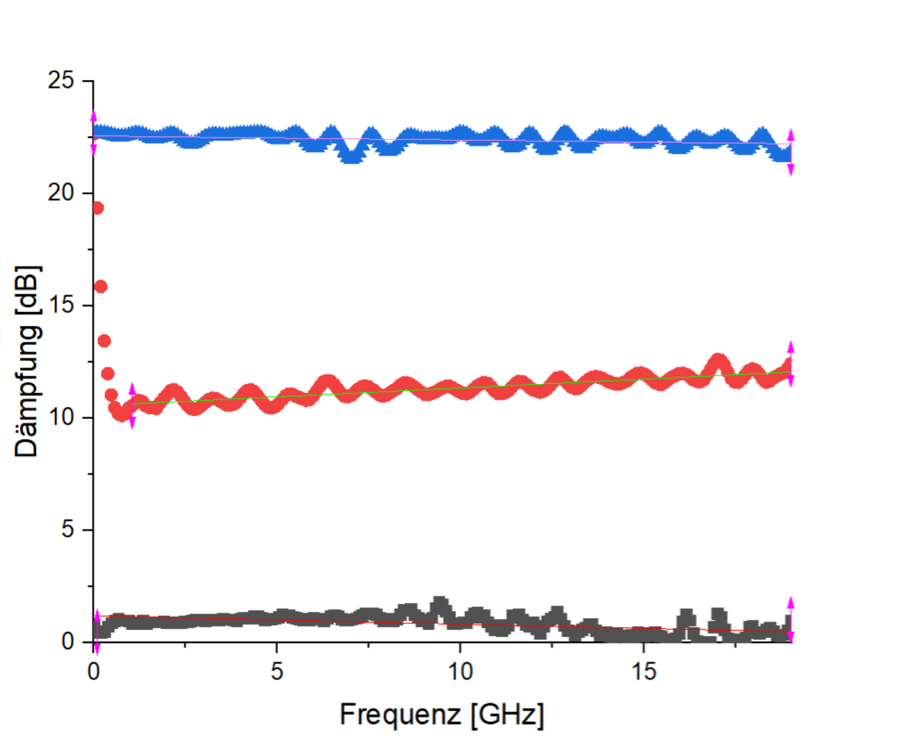
\includegraphics[scale = 1]{Richtkoppler11.png}
	\caption{In schwarz ist die Einfügedämpfung gemessen worden. Diese wurde mit dem orangen Fit mathematisch modelliert. Der Fit ist von der Form $y = a + bx$. Die Fitparameter sind $a = (1,20 \pm 0,04)$dB und $b = (-0,04 \pm 0,004)$dB/Ghz.
	In rot ist die Koppeldämpfung gemessen worden. Diese wurde mit dem grünen Fit mathematisch modelliert. Der Fit ist von der Form $y = a + bx$. Die Fitparameter sind $a = (10,55 \pm 0,04)$dB und $b = (-0,08 \pm 0,003)$dB/Ghz. Die senkrechten Markierungen stellen den Bereich dar, der Modelliert wird.
	In blau ist die Isolation gemessen worden. Diese wurde mit dem rosa Fit mathematisch modelliert. Der Fit ist von der Form $y = a + bx$. Die Fitparameter sind $a = (22,57 \pm 0,03)$dB und $b = (-0,02 \pm 0,003)$dB/Ghz.}
	\label{Richt}
\end{figure}
Auch bei dem Richtkoppler kann erkannt werden, dass die Dämpfung nahe zu konstant sind. Es ist zu beobachten, dass die Isolation die stärkste Dämpfung ist. Das ist deshalb so, da bei der Isolation die Wellen zu einer destruktiven Interferenz geführt werden, somit kann kaum Leistung übertragen werden. Dies ist der Fall, falls man die übertragene Leistung von Tor 2 zu Tor 4 misst, wie es in \cref{IsoF} steht.  Bei der Koppeldämpfung wird  die übertragenen Leistung von Tor 1 zu Tor 4 beobachtet (siehe \cref{KppF}). Hier ist die Dämpfung von Hauptleitung zu Nebenleitung zu sehen. Obwohl hier eine konstruktive Interferenz stattfindet, kommt es zur Dämpfung. Die Einfügedämpfung misst die Dämpfung der übertragenen Leistung von Tor 1 zu Tor 2. Da diese Strecke ohne jegliche Abzweigungen und Interferenzerscheinungen vonstatten geht, ist zu erwarten, dass hier die geringste Dämpfung stattfindet. Tatsächlich finden wir hier den geringsten Wert.

\subsubsection{Zirkulator}
Bei dem Zirkulator wurden zwei verschiedene Bauteile vermessen. Ein großer Zirkulator und ein kleiner Zirkulator. Beide Messkurven die des großen Zirkulators, sowie des kleinen Zirkulators wurde in Durch- und in Sperrrichtung vermessen und in einem Diagramm dargestellt.
\begin{figure}[h!]
	\centering
	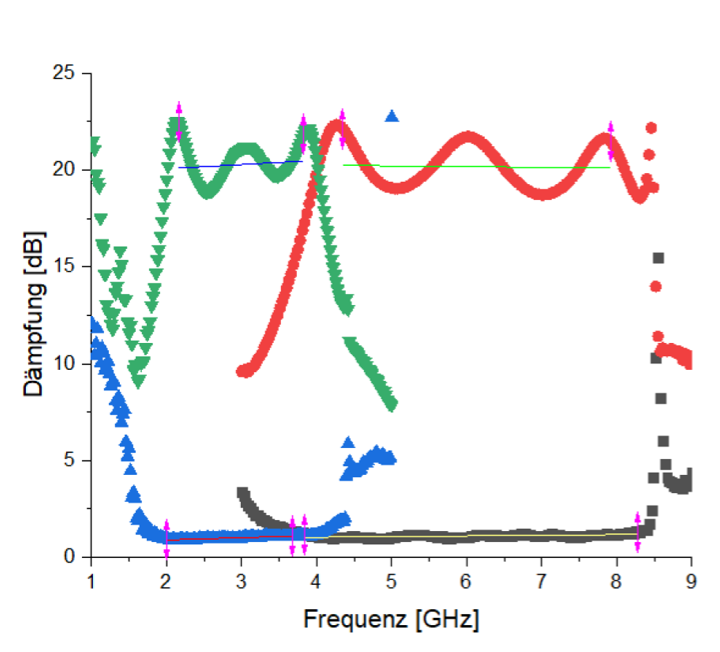
\includegraphics[scale = 1]{Zirkulator11.png}
	\caption{In diesem Bild können zwei Zirkulatoren beobachtet werden die schwarzen sowie die roten Punkte gehören dem kleinen Zirkulator. Die blauen und die grünen Dreiecke gehören zum großen Zirkulator. Die schwarzen und blauen Messwerte beschreiben die Durchlassrichtung und die roten und grünen Punkte die Sperrrichtung. Die senkrechten Markierungen stellen den gefitteten Bereich dar.
	Die jeweiligen Fits sind von der Form $y = a + bx$. 
	Die Durchlassrichtung des kleinen Zirkulators besitzen folgende Fitparameter ($a = (0,89 \pm 0,02)$dB und $b = (-0,03 \pm 0,004)$dB/Ghz.).
	Die Durchlassrichtung des großen Zirkulators besitzen folgende Fitparameter ($a = (0,65 \pm 0,02)$dB und $b = (-0,12 \pm 0,005)$dB/Ghz.).
	Die Sperrrichtung des kleinen Zirkulators besitzen folgende Fitparameter ($a = (20,4 \pm 0,6)$dB und $b = (0,65 \pm 0,02)$dB/GHz).
	Die Sperrrichtung des großen Zirkulators besitzen folgende Fitparameter ($a = (19,6 \pm 0,6)$dB und $b = (0,2 \pm 0,2)$dB/Ghz).}
	\label{ZirkB}
\end{figure}
In dem Diagramm sind zwei verschiedene Zirkulatoren zu sehen. Der heuristische Verlauf beider Graphen ist ähnlich. Beide Verläufe sind außerhalb der Bandbreiten der Sperrrichtung und Durchlassrichtung nicht linear. Innerhalb ihrer Bandbreiten stellen sich Resonanzen heraus, sodass diese sich nur im Mittel zu einer Konstanten ergeben (In diesem Zusammenhang kann von Resonanzen gesprochen werden, da es gesonderte Frequenzen existieren bei denen Maxima auftreten). So stellt der geplottete Verlauf nur eine Näherung in nullter Ordnung dar und vernachlässigt die Dynamik innerhalb der Bandbreiten.
Die Bandbreite beträgt beim kleinen Zirkulator etwa 4GHz bis 8GHz und beim großen Zirkulator etwa 2GHz bis 3,7 GHz. Die einzigen Unterschiede in nullter Ordnung sind die, dass die Bauteile in verschiedenen Bandbreiten funktionieren und die Bandbreiten unterschiedlich groß sind. Die Bandbreite des kleinen Zirkulators ist dabei größer, als die des großen Zirkulators. Das Dämpfungsmaß ist hingegen bei beiden Zirkulatoren in Sperrichtung in Abhängigkeit der Fehler gleich groß und in Durchlassrichtung in Abhängigkeit der Fehler nur in derselben Größenordnung.

\subsection{Ausbreitungsgeschwindigkeit und relative Permittivität}
Im letzten Abschnitt werden Lichtgeschwindigkeit und Permittivität zwei verschiedener Koaxialkabel bestimmt. Zuerst wurde dafür der Abstand zwischen zwei benachbarten Resonanzen bestimmt. In \cref{gleich} sind die Messergebnisse für die Messung mit Kabel 1 sowohl für offenes Kabelende als auch für kurzgeschlossenes Kabelende dargestellt. Dabei ist die Leistung in dBm gegen die Frequenz in GHz aufgetragen.

\begin{figure}[h]
	\centering
	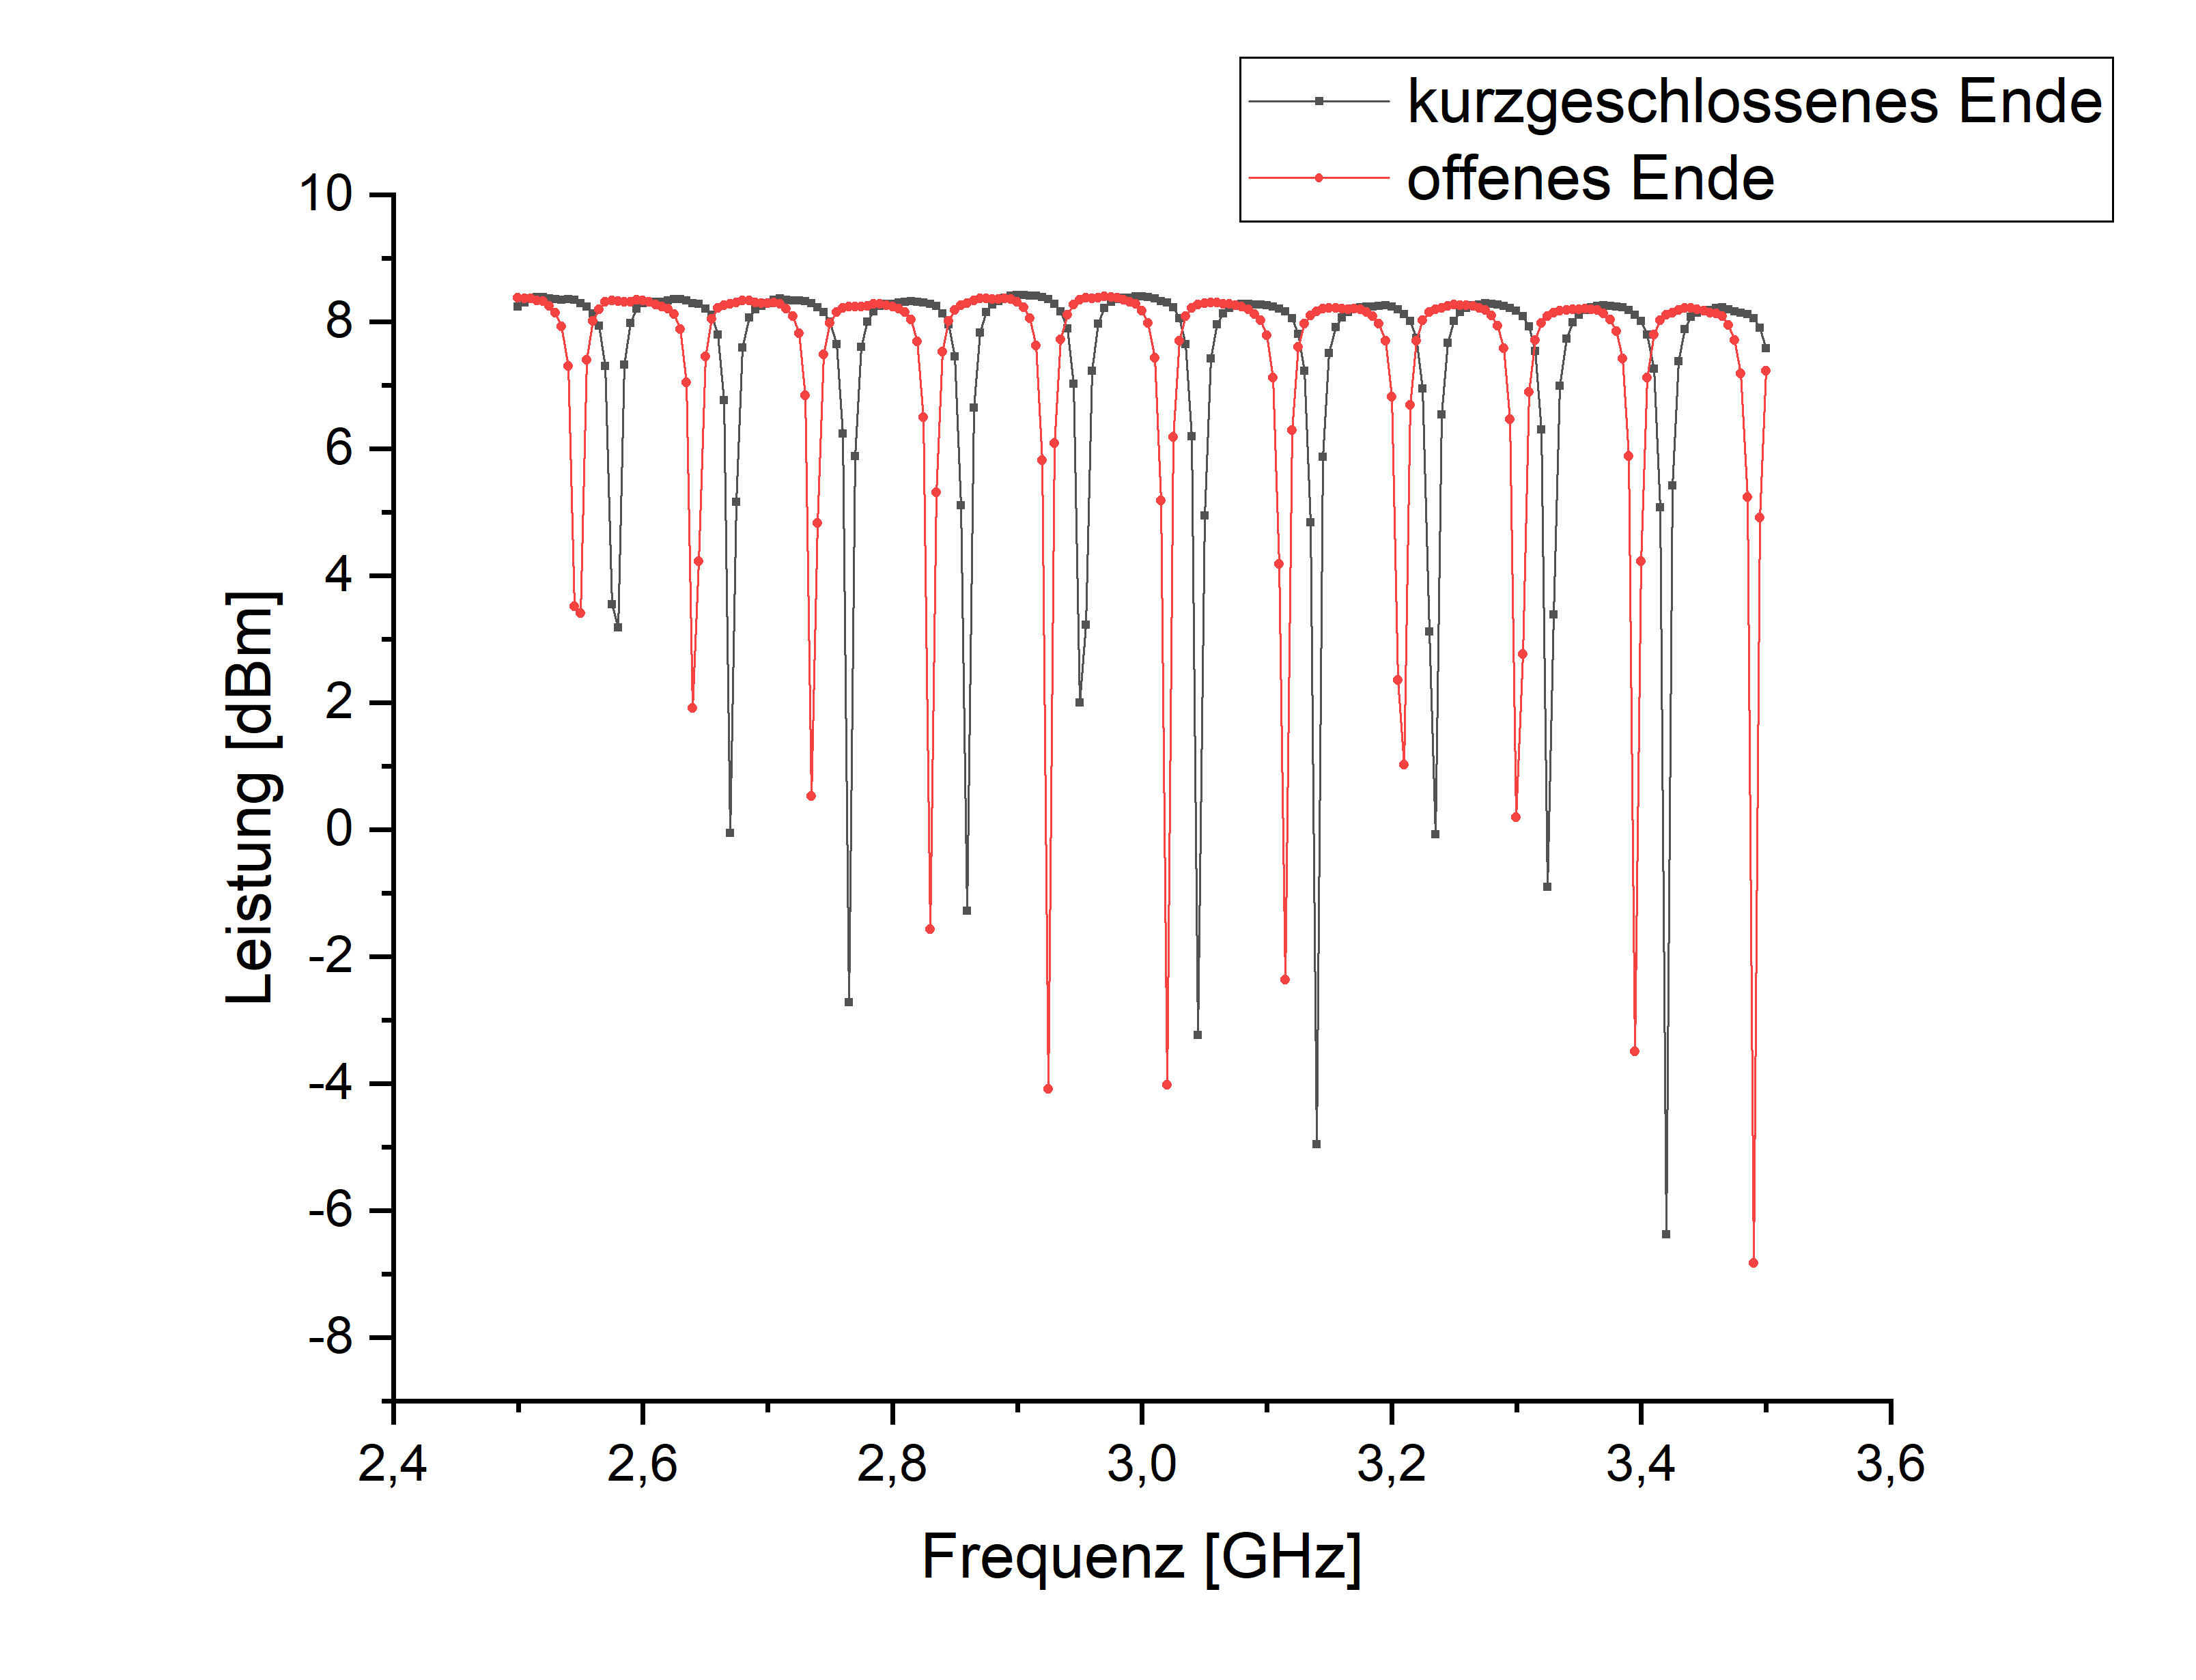
\includegraphics[scale=0.6]{gleiches_Kabel.png}
	\caption{Leistung in Abhängigkeit der Frequenz für offenes und kurzgeschlossenes Kabelende für Kabel 1. Deutlich erkennbar sind die Resonanzfrequenzen.}
	\label{gleich}
\end{figure}

Außerhalb der Resonanzen beträgt die Leistung konstant etwa $\SI{8}{dBm}$, an den Resonanzen fällt sie um mehrere Größenordnungen ab. Für beide Messungen wurde der mittlere Abstand zwischen zwei Resonanzfrequenzen ermittelt. Hierfür wurde der Mittelwert aus allen Frequenzabständen benachbarter Resonanzen gebildet.

\begin{figure}[h]
	\centering
	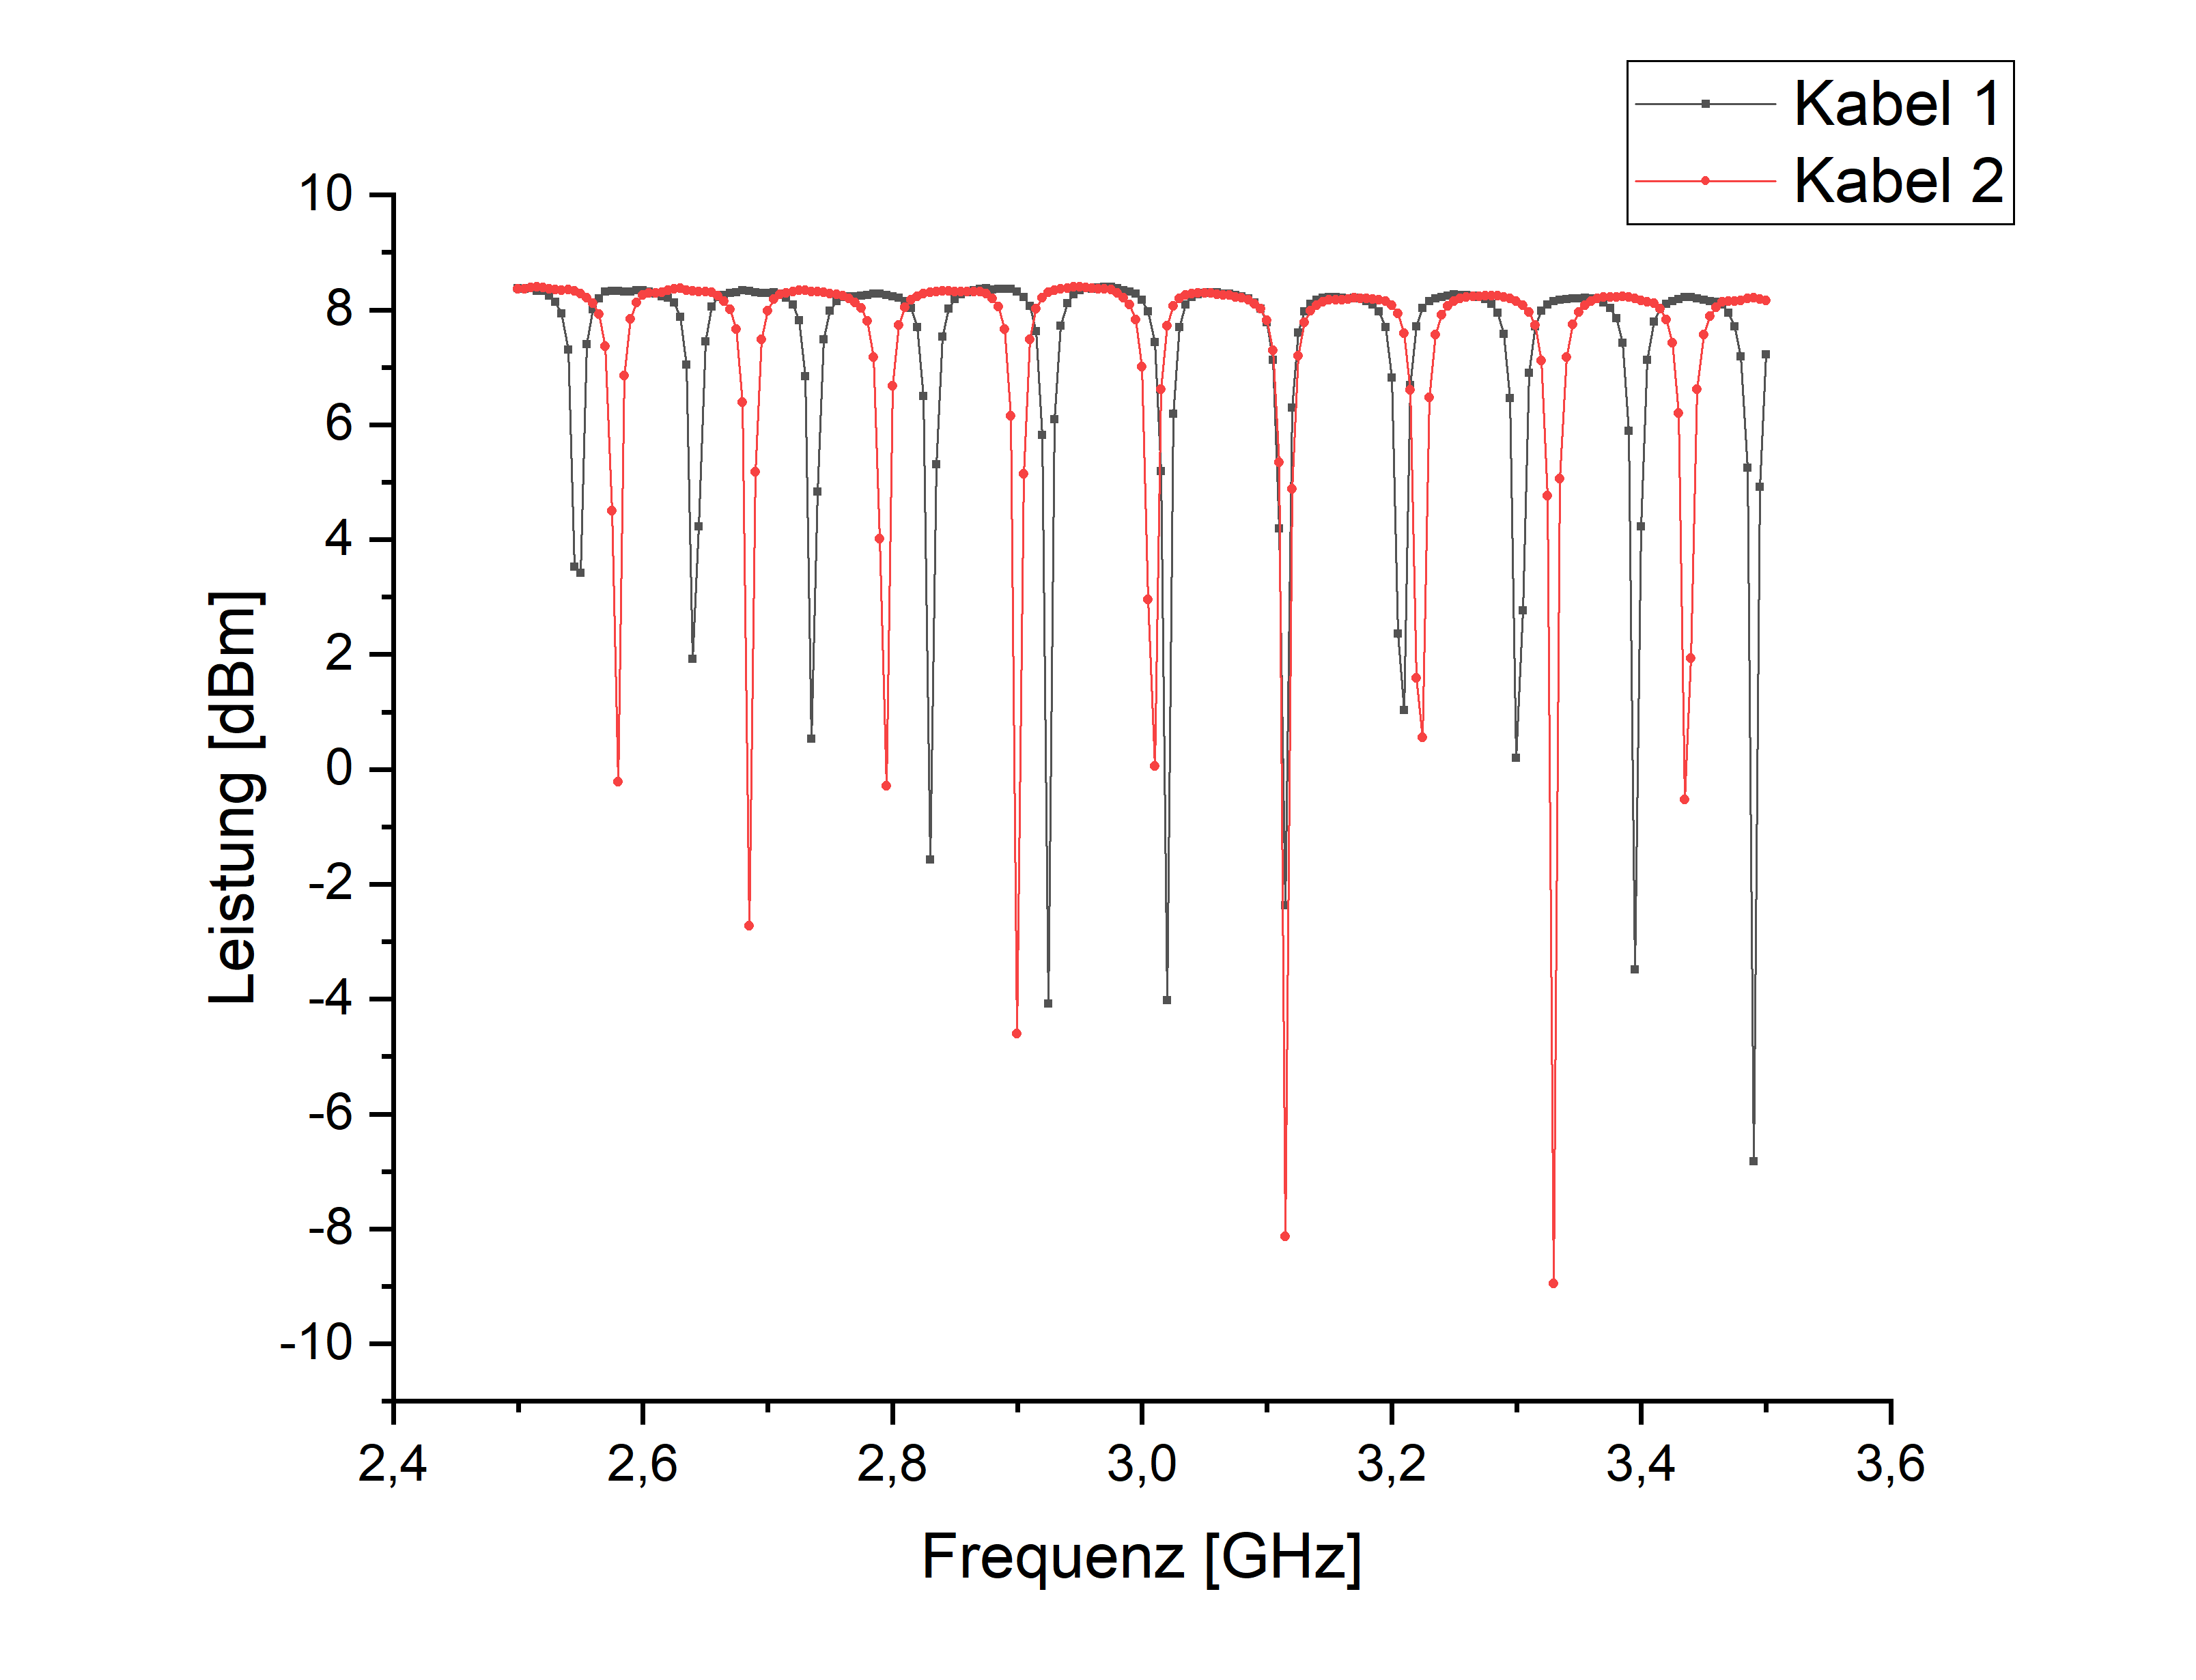
\includegraphics[scale=0.6]{anderes_Kabel.png}
	\caption{Leistung in Abhängigkeit der Frequenz für offenes Kabelende für Kabel 1 und 2. Deutlich erkennbar sind die unterschiedlichen Abstände zwischen den Resonanzen.}
	\label{anderes}
\end{figure}

Es ergeben sich Werte von $\SI{0,094\pm0,002}{GHz}$ für das offene Kabelende und $\SI{0,093\pm0,002}{GHz}$ für das geschlossene Kabelende. Die Unsicherheit ergeben sich aus direkt aus der Standardabweichung vom Mittelwert. Die Fehler der Geräte liegen unter $0,01\%$ und können daher vernachlässigt werden. Der mittlere Abstand der beiden Resonanzfrequenzen ist im Rahmen der Unsicherheit gleich. Die Art des Abschlusswiderstands hat damit offenbar keine Auswirkung auf den Abstand der Resonanzen. Allerdings treten die Resonanzen bei kurzgeschlossenem Ende jeweils bei um etwa $\SI{300}{MHz}$ höheren Frequenzen auf als die Resonanzen bei offenem Ende.

Für ein anderes Kabel (im folgenden Kabel 2) wurde anschließend die gleiche Messung mit offenem Ende durchgeführt. In \cref{anderes} werden die Ergebnisse der Messungen mit offenem Ende beider Kabel verglichen. Direkt erkennbar ist, dass hier der Abstand zwischen zwei Resonanzen unterschiedlich ist.


Auf die gleiche Weise wie oben wurde anschließend der mittlere Abstand zweier benachbarter Resonanzen bestimmt, hierfür ergibt sich ein Wert von $\SI{0,106\pm0,002}{GHz}$. Dieser ist signifikant größer als der von Kabel 1. Aus den mittleren Frequenzabständen kann nun mit \cref{eq:c} die Ausbreitungsgeschwindigkeit der Wellen im Koaxialkabel bestimmt werden. Die hierfür erforderliche Länge des Kabel wurde mit einem Maßband gemessen. Es ergibt sich für Kabel 1 bei offenem Ende ein Wert von $\SI{235000\pm5088}{km/h}$ und bei kurzgeschlossenem Ende ein Wert von $\SI{233333\pm5966}{km/h}$.Wie erwartet ist die Ausbreitungsgeschwindigkeit der Welle im Kabel unabhängig vom gewählten Abschlusswiderstand. Für Kabel 2 ergibt sich ein Wert von $\SI{254363\pm5859}{km/h}$. Die Unsicherheiten wurden über die Fehlerfortpflanzung mit \cref{eq:uc} berechnet.

\begin{equation}
	u(c) = \sqrt{\left( 2u(l)\Delta f\right) ^2 +\left( 2u(\Delta f)l\right) ^2}
	\label{eq:uc}
\end{equation}

Mithilfe der Ausbreitungsgeschwindigkeit kann nun über \cref{eq:er} die relative Permittivität bestimmt werden. Diese beträgt für Kabel 1 $\SI{1,627\pm0,070}{}$ bei offenem Ende bzw. $\SI{1,651\pm0,084}{}$. Es besteht also auch hier kein Unterschied bei verschiedenen Abschlusswiderständen. Für Kabel 2 beträgt die relative Permittivität $\SI{1,389\pm0,064}{}$. Die Unsicherheit wurde mit \cref{eq:uer} bestimmt.

\begin{equation}
	u(\epsilon_r) = \frac{2u(c)c^2}{c^3}
	\label{eq:uer}
\end{equation}

\section{Diskussion}
Es konnte eine Charakterisierung aller vorhandenen Bauteile durchgeführt werden. Die Sperr- und Durchlassrichtungen der Bauteile ergaben in ihrer Bandbreite Geraden mit geringer Steigung. Bei den Zirkulatoren gab es innerhalb der Bandbreite Resonanzen, sodass hier allerhöchstens qualitativ eine Aussage getroffen werden konnte. Dennoch war ein klarer Unterschied der Dämpfung bei Sperr- und Durchlassrichtung zu erkennen. Ein weiterer Effekt, welcher erst im Laufe des Berichtes korrigiert wurde, war der, wie bereits oben erwähnte, kurze Draht mit einer starken Biegung. Dieser wurde später durch einen längeren ersetzt. Durch die starke Biegung des Drahtes kam es zur Reflexion. So beobachtet man Resonanzen in den ersten Charakterisierungen der Bauteile. Diese Resonanzen wären nicht aufgetreten, wenn von vornherein ein längerer Kabel genutzt werden würde. 

Wie erwartet war sowohl der Frequenzabstand zwischen zwei Resonanzen, als auch die Ausbreitungsgeschwindigkeit und die relative Permittivität unabhängig von der Wahl des Abschlusswiderstands. Dieser sorgte nur für eine Verschiebung der Resonanzen um einige $100$ MHz. Da die beiden Kabel unterschiedliche Ausbreitungsgeschwindigkeiten und relative Permittivitäten besitzen, bestehen sie offenbar aus unterschiedlichen Stoffen oder eins der Kabel ist beschädigt oder verunreinigt. 